\documentclass[12pt]{article}

\usepackage{sbc-template}
\usepackage{graphicx,url}
\usepackage[utf8]{inputenc}
\usepackage[T1]{fontenc}
\usepackage[brazil]{babel}
\usepackage{tikz}
\usetikzlibrary{arrows.meta,positioning,shapes.geometric}

\sloppy

\title{Detecção de Imagens Sintéticas após Transformações Digitais}

\author{Nathália G. Ribas\inst{1}, Igor M. da Rosa\inst{1}}

\address{Departamento de Computação (DEC)\\
Universidade Federal de Santa Catarina\\
Araranguá, SC
\email{ribas.nathalia@grad.ufsc.br, igor.matos.rosa@grad.ufsc.br}
}

\begin{document}

\maketitle

\begin{abstract}
This work studies how classical computer vision methods behave when detecting AI-generated images that go through common digital transformations, such as JPEG compression, crop, resize and blur. Frequency, spatial and texture descriptors (FFT, HOG and LBP) are reviewed, together with SVM, $k$-NN and convolutional networks. Two training protocols are compared. Training only on original CIFAKE images yields 92.04\% fusion accuracy on the clean test, but the detector collapses to about 54\% after crop, blur or a combined pipeline --- repeating the ZeroGPT failure. Including the nine transforms in training trades some clean-test accuracy (86.08\%) for robustness: fusion remains above 71\% after the same pipeline.
\end{abstract}

\begin{resumo}
Este trabalho estuda como métodos clássicos de visão computacional se comportam ao detectar imagens geradas por IA depois de transformações digitais comuns, como compressão JPEG, crop, resize e blur. Revisam-se descritores de frequência, espaço e textura (FFT, HOG e LBP) e os classificadores SVM, $k$-NN e redes convolucionais. Comparam-se dois protocolos de treino. Treinar só nas originais do CIFAKE rende 92,04\% de fusão no teste limpo, mas o detector cai para cerca de 54\% após crop, blur ou o pipeline combinado --- o mesmo tipo de falha observado no ZeroGPT. Incluir as nove transformações no treino reduz a acurácia no original para 86,08\% e mantém a fusão acima de 71\% após o mesmo pipeline.
\end{resumo}

%----------------------------------------------------------------------
\section{Introdução}
%----------------------------------------------------------------------

Hoje é fácil gerar imagens realistas com inteligência artificial, o que dificulta saber se uma foto é verdadeira ou criada por um modelo. Em situações práticas --- como posts em redes sociais em período eleitoral ou anúncios de imóveis --- essas imagens quase nunca chegam intactas: passam por compressão, corte, redimensionamento e filtros. Essas mudanças podem enfraquecer os sinais que os detectores usam para reconhecer conteúdo sintético.

A pergunta deste trabalho é: \emph{quão bem detectores baseados em features clássicas continuam funcionando quando a imagem sofre transformações típicas da internet?} Em vez de só classificar ``real versus IA'' em imagens limpas, o foco é um teste de robustez em dois passos: primeiro treinar só no original e medir a queda --- o mesmo tipo de falha do ZeroGPT ---; depois treinar também com as transformações e verificar se o detector deixa de colapsar.

Um teste inicial com o site ZeroGPT\footnote{\url{https://www.zerogpt.com/pt/ai-image-detector}} ajuda a ilustrar o problema. Partindo de uma foto real de estúdio, pediu-se a uma IA para mudar a cena (mantendo a pessoa). O ZeroGPT marcou a imagem editada como cerca de 99\% falsa. Depois, apenas comprimindo essa mesma imagem, o resultado passou para cerca de 97\% real --- ou seja, a manipulação deixou de ser detectada (Figura~\ref{fig:zerogpt-editada}).

\begin{figure}[ht]
\centering
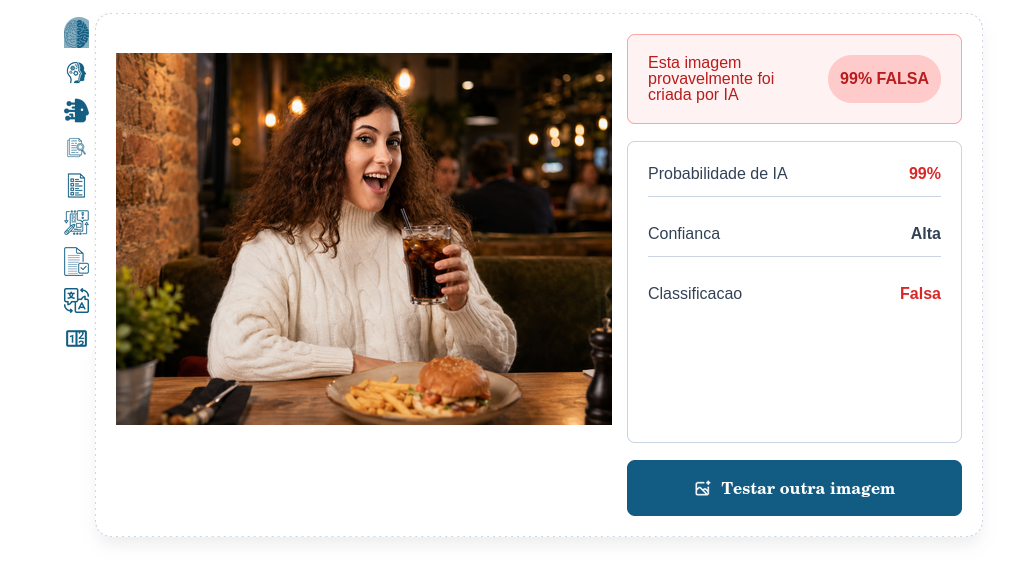
\includegraphics[width=0.48\textwidth]{../../exemplos/editada_ia/TestePosTransformacao.png}
\hfill
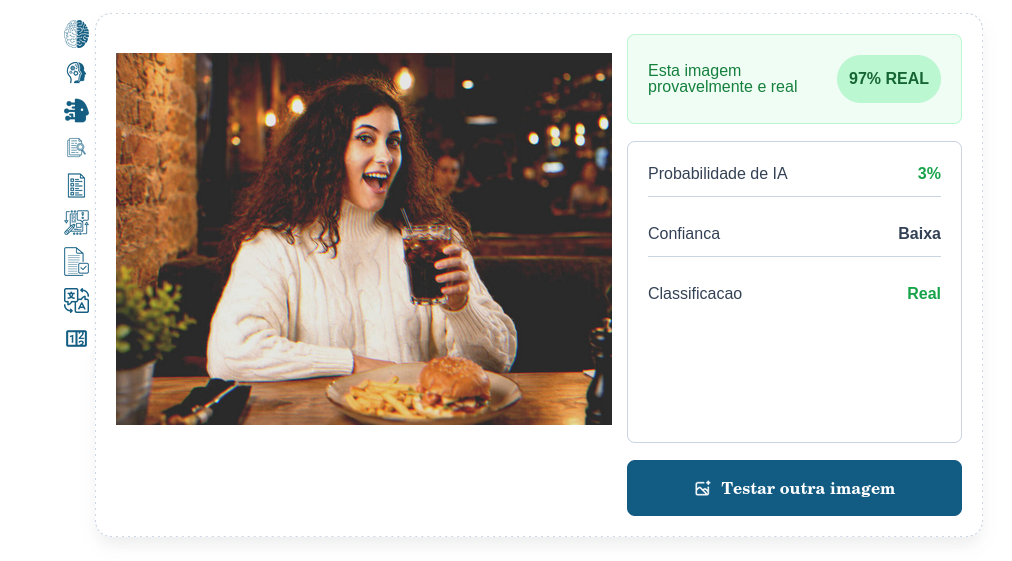
\includegraphics[width=0.48\textwidth]{../../exemplos/editada_ia/TesteReducaoReso.png}
\caption{Resultados do ZeroGPT. À esquerda: foto real com cena alterada por IA ($\approx$99\% falsa). À direita: a mesma imagem após compressão ($\approx$97\% real), mostrando que o detector falhou.}
\label{fig:zerogpt-editada}
\end{figure}

%----------------------------------------------------------------------
\section{Trabalhos Relacionados}
%----------------------------------------------------------------------

Vários trabalhos já tratam da detecção de imagens geradas por IA, usando datasets públicos, análise em frequência, features manuais ou redes neurais.

Bird e Lotfi~\cite{bird2024cifake} criaram o CIFAKE, com imagens reais do CIFAR-10 e imagens sintéticas feitas com Stable Diffusion, e obtiveram cerca de 93\% de acurácia com CNN. Esse dataset é a base deste projeto, por ser balanceado, bem documentado e já usado em estudos com features manuais~\cite{nirob2026handcrafted}.

Frank et al.~\cite{frank2020frequency} mostraram que imagens de GANs deixam marcas claras no espectro de frequência, ligadas ao \emph{upsampling}, o que ajuda a separar real de fake e ainda resiste melhor a blur e crop. Bammey~\cite{bammey2024synthbuster} levou essa ideia para modelos de difusão (Synthbuster), olhando picos no espectro de Fourier e conseguindo detectar imagens mesmo com JPEG leve. Por isso faz sentido empregar features de frequência e testar compressão JPEG neste trabalho.

Nirob et al.~\cite{nirob2026handcrafted} testaram várias features manuais no CIFAKE (histograma, DCT, HOG, LBP, GLCM, wavelets) com classificadores clássicos e ensembles. A combinação de features teve bom desempenho, o que reforça o uso de FFT, HOG e LBP.

Choi et al.~\cite{choi2025warpad} propuseram o WaRPAD, um método sem treino específico que mede o quanto embeddings mudam com crop/resize. Embora a técnica seja distinta da abordada aqui, o trabalho mostra que transformações geométricas prejudicam a detecção --- o mesmo tipo de degradação que se pretende medir.

Em resumo: (i)~frequência e textura ajudam na detecção~\cite{frank2020frequency,bammey2024synthbuster,nirob2026handcrafted}; (ii)~é importante testar transformações realistas~\cite{choi2025warpad,bammey2024synthbuster}. O objetivo é medir, com features clássicas e SVM no CIFAKE, quanto cada transformação e cada tipo de feature perde desempenho.

%----------------------------------------------------------------------
\section{Fundamentação Teórica}
\label{sec:fundamentacao}
%----------------------------------------------------------------------

Esta seção descreve as técnicas e os algoritmos estudados para o problema. A justificativa da escolha de uma delas e a perspectiva de utilização no projeto constam da Seção~\ref{sec:desenvolvimento}.

\subsection{Visão clássica e aprendizado profundo}

Há dois caminhos principais para decidir se uma imagem é real ou gerada por IA.

Na \emph{visão clássica}, a imagem é resumida por descritores calculados explicitamente (frequência, bordas, textura) e um classificador --- SVM ou $k$-NN --- aprende a fronteira entre as classes~\cite{gonzalez2018,nirob2026handcrafted}. Cada componente do vetor tem interpretação visual, o que permite relacionar uma transformação (JPEG, crop, blur) à degradação de um domínio específico.

No \emph{aprendizado profundo}, uma rede convolucional (CNN) aprende os padrões internamente. No CIFAKE, esse tipo de modelo atinge cerca de 93\% de acurácia~\cite{bird2024cifake}. A contrapartida é a menor transparência: torna-se mais difícil associar a queda de desempenho ao domínio de valor, de espaço ou de frequência.

Como o problema em estudo é de \emph{robustez interpretável} --- não apenas classificar, mas indicar \emph{qual padrão se perde} após cada transformação --- as duas famílias foram consideradas. A via clássica permanece como eixo do projeto.

\subsection{Domínio da frequência: FFT}

Uma imagem pode ser vista como soma de ondas de diferentes frequências~\cite{gonzalez2018}. A Transformada Rápida de Fourier (FFT) decompõe essa soma. O espectro de magnitude indica a contribuição de cada frequência: o centro concentra variações suaves (baixa frequência) e as bordas, detalhes e ruído (alta frequência).

Na detecção de conteúdo sintético, esse domínio é relevante porque o processo de geração --- em especial o \emph{upsampling} de GANs e de modelos de difusão --- deixa marcas periódicas no espectro~\cite{frank2020frequency,bammey2024synthbuster}. A compressão JPEG também atua em frequência, ao descartar coeficientes de alta frequência. A FFT é, portanto, candidata tanto à detecção quanto à análise do efeito do JPEG.

Operacionalmente, aplica-se a FFT 2D à imagem em escala de cinza, desloca-se o espectro para centralizar as baixas frequências, toma-se a magnitude em escala logarítmica e reduz-se o mapa 2D a um vetor 1D por média radial em anéis de frequência. Esse vetor é o descritor apresentado ao classificador.

\subsection{Domínio do espaço: HOG}

O Histograma de Gradientes Orientados (HOG) descreve a forma local da imagem~\cite{dalal2005hog}. Em cada região, mede-se a orientação das bordas (horizontal, vertical, diagonal) e acumulam-se essas direções em um histograma. A concatenação dos histogramas das células resume o desenho da cena, independentemente da cor.

O descritor foi proposto originalmente para detecção de pessoas, mas é um padrão do domínio espacial e já foi avaliado no CIFAKE com features manuais~\cite{nirob2026handcrafted}. Recorte e redimensionamento alteram a geometria das bordas; o blur as suaviza. HOG é, portanto, o descritor adequado para observar o efeito de crop, resize e filtros de suavização.

\subsection{Domínio da textura: LBP e GLCM}

O Padrão Binário Local (LBP) descreve a textura comparando cada pixel com os vizinhos em um círculo~\cite{ojala2002lbp}. Se o vizinho é mais claro, atribui-se 1; se é mais escuro, 0. O código binário rotula o padrão local. O histograma desses rótulos, na versão \emph{uniforme} --- invariante a rotação e com número reduzido de bins --- constitui o vetor de features.

A Matriz de Co-ocorrência de Níveis de Cinza (GLCM) é outra representação clássica de textura: contabiliza pares de pixels a uma dada distância e direção~\cite{gonzalez2018,nirob2026handcrafted}. Foi estudada por integrar o conjunto de descritores manuais relatados no CIFAKE. O LBP, no entanto, tem custo computacional menor e produz um vetor curto, o que é vantajoso quando se treina um SVM em dezenas de milhares de imagens.

Compressão e blur alteram a relação entre um pixel e sua vizinhança; espera-se, portanto, degradação de LBP e de GLCM sob JPEG forte e sob suavização.

\subsection{Classificadores estudados}

Com o vetor de features definido, três famílias de classificador foram examinadas.

\paragraph{SVM.}
A Máquina de Vetores de Suporte busca a fronteira que melhor separa as duas classes, maximizando a margem~\cite{cortes1995svm}. Com kernel linear, a fronteira é um hiperplano; com kernel RBF (\emph{Radial Basis Function}), pode ser curva, o que é adequado quando as classes não são linearmente separáveis. O parâmetro $C$ regula o compromisso entre margem e erros no treino. O SVM é o classificador clássico de reconhecimento de padrões e opera de forma natural sobre vetores de tamanho fixo.

\paragraph{$k$-NN.}
O classificador dos $k$ vizinhos mais próximos atribui à amostra nova o rótulo majoritário entre os $k$ exemplos de treino mais próximos~\cite{cover1967knn}. A regra é transparente, porém a predição, na forma ingênua, percorre o conjunto de treino. Com cerca de 100 mil imagens e vetores de centenas de dimensões, o custo torna-se elevado. Além disso, o método é sensível à escala das features.

\paragraph{CNN e ensembles.}
Redes convolucionais aprendem filtros e alcançam acurácia elevada no CIFAKE~\cite{bird2024cifake}. Ensembles sobre features manuais, como LightGBM, também constam da literatura~\cite{nirob2026handcrafted}. Ambos foram estudados como referência de desempenho. A CNN, contudo, dificulta associar o erro a FFT, HOG ou LBP; o ensemble afasta-se do classificador clássico de margem máxima.

%----------------------------------------------------------------------
\section{Desenvolvimento}
\label{sec:desenvolvimento}
%----------------------------------------------------------------------

A partir das técnicas da Seção~\ref{sec:fundamentacao}, esta seção apresenta a técnica selecionada, a justificativa da escolha, a perspectiva de utilização no problema de robustez e a metodologia do experimento. O fluxo geral está na Figura~\ref{fig:fluxo}. Os números de treino e teste constam da Seção~\ref{sec:resultados}.

\begin{figure}[ht]
\centering
\begin{tikzpicture}[
  node distance=0.55cm and 0.35cm,
  box/.style={draw, rounded corners, align=center, font=\footnotesize,
              inner sep=4pt, minimum width=2.8cm},
  dec/.style={draw, diamond, aspect=2.4, align=center, font=\scriptsize,
              inner sep=1pt},
  arr/.style={-{Latex}, thick}
]
  \node[box, fill=gray!15] (d) {CIFAKE\\real / fake};
  \node[box, below=of d] (f) {Extrair FFT,\\HOG e LBP};
  \node[box, below=of f] (t) {Treinar SVM RBF\\(só originais)};
  \node[box, below=of t] (x) {Testar após\\transformações};
  \node[box, below=of x] (e) {Medir acurácia\\por feature};
  \node[dec, below=0.65cm of e] (q) {Resultado\\aceitável?};
  \node[box, below left=0.75cm and 0.05cm of q, fill=green!12] (ok) {Analisar e\\relatar};
  \node[box, below right=0.75cm and 0.05cm of q, fill=orange!15] (aj) {Ajustar\\features};

  \draw[arr] (d) -- (f);
  \draw[arr] (f) -- (t);
  \draw[arr] (t) -- (x);
  \draw[arr] (x) -- (e);
  \draw[arr] (e) -- (q);
  \draw[arr] (q) -- node[left, font=\scriptsize] {sim} (ok);
  \draw[arr] (q) -- node[right, font=\scriptsize] {não} (aj);
  \draw[arr] (aj.east) -- ++(0.5,0) |- (f.east);
\end{tikzpicture}
\caption{Fluxograma no CIFAKE: a primeira versão treina só no original; se a robustez for baixa, o ajuste inclui as transformações no treino.}
\label{fig:fluxo}
\end{figure}

\subsection{Justificativa da técnica selecionada}

A técnica selecionada combina os descritores \textbf{FFT}, \textbf{HOG} e \textbf{LBP}, concatenados em um único vetor (fusão), com um \textbf{SVM de kernel RBF}.

Os três descritores cobrem os domínios de frequência, espaço e textura e já constam da literatura de detecção~\cite{frank2020frequency,bammey2024synthbuster,nirob2026handcrafted,dalal2005hog,ojala2002lbp}. A FFT captura marcas de geração e o efeito do JPEG; o HOG, a geometria das bordas; o LBP, a textura local. Isolado, cada descritor responde a um tipo de transformação; em conjunto, o classificador dispõe de um retrato mais completo da imagem. Nirob et al.~\cite{nirob2026handcrafted} mostraram que a fusão de descritores manuais no CIFAKE melhora o desempenho, o que justifica concatenar as três representações em vez de restringir o detector a uma única família.

O SVM é preferível ao $k$-NN e à CNN por três razões. Primeiro, trata-se do classificador clássico de margem máxima, com interpretação geométrica clara~\cite{cortes1995svm}. Segundo, com vetor de fusão de 362 dimensões e 100 mil exemplos de treino, o $k$-NN torna a predição custosa e permanece sensível à escala das variáveis. Terceiro, a CNN, ainda que competitiva no CIFAKE~\cite{bird2024cifake}, não expõe de forma direta qual domínio degradou após crop ou JPEG --- precisamente o que o protocolo de robustez precisa evidenciar. O kernel RBF, em detrimento do kernel linear, admite fronteira não linear, hipótese mais realista para a separação real/sintético em features manuais.

GLCM, histograma de cor e DCT foram estudados~\cite{nirob2026handcrafted,gonzalez2018}, mas não integram o pipeline principal: repetiriam informação já coberta por LBP (textura) e por FFT (frequência), além de aumentar a dimensionalidade sem ganho interpretativo proporcional.

\subsection{Perspectiva de utilização no problema}

O problema específico não se reduz a classificar uma imagem intacta. Interessa saber se o detector permanece eficaz depois que a imagem circula em redes sociais, ou seja, depois de compressão, recorte, redimensionamento e filtros. Dois protocolos respondem a essa pergunta.

No primeiro, o SVM \emph{não} é treinado em imagens transformadas. A fronteira real/sintético é aprendida apenas nas originais do CIFAKE e permanece fixa na avaliação. O que se altera é o conjunto de teste. Esse desenho mede a \emph{queda} de acurácia e reproduz, de forma controlada, a falha do ZeroGPT: um detector que acerta a imagem limpa e deixa de detectar depois de uma transformação banal.

Quando essa queda se mostra inaceitável, o segundo protocolo inclui as nove transformações no treino, todas com o mesmo rótulo real/sintético. A fronteira passa a ver JPEG, crop, resize, blur e o pipeline já no treino, o que se aproxima do uso prático. A avaliação continua sem retreino: as mesmas imagens de teste são apresentadas intactas e após cada transformação.

Essa leitura associa cada descritor a um mecanismo de degradação esperado:

\begin{itemize}
\item JPEG altera o espectro e deve afetar sobretudo a FFT~\cite{bammey2024synthbuster};
\item crop e resize modificam a geometria e devem afetar o HOG~\cite{choi2025warpad,dalal2005hog};
\item blur e compressão forte perturbam a vizinhança dos pixels e devem afetar o LBP~\cite{ojala2002lbp}.
\end{itemize}

A fusão corresponde ao detector de uso prático, destinado a uma imagem qualquer. FFT, HOG e LBP isolados permanecem no experimento para localizar \emph{onde} a robustez se perde. Se a acurácia da fusão for insuficiente, ajustam-se descritores ou hiperparâmetros e o ciclo da Figura~\ref{fig:fluxo} se repete. Os resultados dessa avaliação constam da Seção~\ref{sec:resultados}.

A mesma cadeia --- extração dos três descritores, fusão e SVM já treinado --- admite, como desdobramento, uma ferramenta de inspeção que recebe uma imagem e devolve um escore de probabilidade de conteúdo sintético, inclusive após as transformações do protocolo.

\subsection{Metodologia}

O experimento emprega o CIFAKE~\cite{bird2024cifake} na divisão original, resolução $32{\times}32$, classes balanceadas (reais provenientes do CIFAR-10 e sintéticas geradas por Stable Diffusion). Não há coleta própria. Os exemplos do ZeroGPT (Figura~\ref{fig:zerogpt-editada}) não participam do cálculo das métricas; servem apenas para motivar o problema. O teste é o CIFAKE completo: 20 mil imagens, em ambos os protocolos.

Na versão~1, o SVM treina em 100 mil imagens originais. Na versão~2, utilizam-se 5 mil imagens por classe (10 mil imagens-base); cada uma gera 10 amostras --- original mais as nove transformações --- totalizando também 100 mil exemplos. O volume de treino permanece comparável; o que muda é a presença das variantes digitais.

A FFT é calculada em escala de cinza, com deslocamento do espectro, magnitude logarítmica e média radial em 64 faixas, gerando um vetor de 64 componentes normalizado em $[0,1]$. O HOG utiliza células $8{\times}8$, blocos $2{\times}2$ e 8 orientações, parâmetros adequados a $32{\times}32$~\cite{dalal2005hog}, e produz 288 componentes. O LBP uniforme emprega $P=8$ vizinhos e raio $R=1$, com histograma de 10 bins normalizado~\cite{ojala2002lbp}. Cada família é padronizada por \texttt{StandardScaler} ajustado exclusivamente no treino, a fim de evitar vazamento de informação do teste e de impedir que a dimensionalidade maior de um descritor domine o SVM. A fusão concatena os três vetores já escalados, na ordem FFT, HOG e LBP, totalizando 362 componentes.

Treina-se um SVM por descritor isolado, para comparar os domínios, e um SVM sobre a fusão, para maximizar o desempenho conjunto. Em todos os casos utiliza-se \texttt{SVC} com kernel RBF, $C=10$ e $\gamma=\mathrm{scale}$~\cite{cortes1995svm}. Busca em grade de $C$ restringe-se a subconjuntos menores; no conjunto completo o valor permanece fixo, pois validação cruzada com RBF em 100 mil exemplos seria incompatível com o tempo disponível. Modelos e scalers são persistidos para reutilização na avaliação e em eventuais ferramentas de inspeção.

As transformações reproduzem a circulação digital~\cite{bammey2024synthbuster,choi2025warpad}: JPEG com qualidade 90, 70 e 50; crop aleatório de 10\%, 25\% e 40\%, com retorno a $32{\times}32$; redução à metade da resolução e restauração do tamanho; blur gaussiano $3{\times}3$; e o pipeline \emph{crop 25\% $\rightarrow$ resize $0{,}5$ $\rightarrow$ JPEG 70}. Após cada operação a imagem permanece RGB $32{\times}32$, de modo que a dimensionalidade dos descritores não se altere.

A métrica principal é a acurácia. Em cada versão compara-se o teste original (baseline) com o teste transformado, para FFT, HOG, LBP e fusão, sem retreinar o classificador. Gráficos de barras da acurácia subsidiam a discussão sobre quais padrões visuais desaparecem com cada transformação e sobre o ganho da versão~2 em relação à versão~1.

%----------------------------------------------------------------------
\section{Resultados}
\label{sec:resultados}
%----------------------------------------------------------------------

Os dois protocolos usam o mesmo SVM RBF ($C=10$), as mesmas features e o mesmo teste de 20 mil imagens. O que muda é o treino.

\subsection{Versão 1: treino só no original}

A Tabela~\ref{tab:svm-v1} mostra o teste original. A fusão atinge 92,04\%, acima de HOG (81,77\%), FFT (80,74\%) e LBP (72,12\%). No original, o detector clássico funciona.

\begin{table}[ht]
\centering
\caption{Versão 1 --- SVM RBF no teste original. Treino: 100 mil imagens intactas.}
\label{tab:svm-v1}
\begin{tabular}{lrrr}
\hline
Feature & Acurácia & Tempo (s) & Tempo (h) \\
\hline
FFT    & 0,8074 & 959,0   & 0,27 \\
HOG    & 0,8177 & 12100,6 & 3,36 \\
LBP    & 0,7212 & 176,0   & 0,05 \\
Fusão  & 0,9204 & 5555,6  & 1,54 \\
\hline
\end{tabular}
\end{table}

A Tabela~\ref{tab:transf-v1} e a Figura~\ref{fig:acuracia-v1} mostram o mesmo classificador, sem retreino, no teste transformado. JPEG 90 e 70 quase não alteram a fusão (91,53\%). JPEG 50 cai para 86,11\%. Crop, resize, blur e o pipeline reproduzem a falha do ZeroGPT: a fusão despenca para 62,41\% (crop 10\%), 56,52\% (crop 25\%), 55,24\% (crop 40\%), 55,13\% (resize), 55,18\% (pipeline) e 53,71\% (blur). O detector acerta a foto limpa e deixa de distinguir real de sintético depois de uma alteração banal.

\begin{table}[ht]
\centering
\caption{Versão 1 --- acurácia no teste transformado, sem retreinar. Treino apenas em originais.}
\label{tab:transf-v1}
\setlength{\tabcolsep}{4.5pt}
\begin{tabular}{lcccc}
\hline
Transformação & FFT & HOG & LBP & Fusão \\
\hline
original     & 0,8074 & 0,8177 & 0,7212 & 0,9204 \\
JPEG 90      & 0,7956 & 0,8165 & 0,7153 & 0,9153 \\
JPEG 70      & 0,7877 & 0,8148 & 0,7197 & 0,9153 \\
JPEG 50      & 0,6364 & 0,7980 & 0,7000 & 0,8611 \\
crop 10\%    & 0,5211 & 0,7517 & 0,6497 & 0,6241 \\
crop 25\%    & 0,5082 & 0,6722 & 0,6031 & 0,5652 \\
crop 40\%    & 0,4782 & 0,6238 & 0,5548 & 0,5524 \\
resize $0{,}5$ & 0,5170 & 0,7581 & 0,5847 & 0,5513 \\
blur $3{\times}3$ & 0,5093 & 0,7830 & 0,6236 & 0,5371 \\
pipeline     & 0,4725 & 0,6387 & 0,5380 & 0,5518 \\
\hline
\end{tabular}
\end{table}

\begin{figure}[ht]
\centering
\includegraphics[width=\textwidth]{../../cod/results/acuracia_por_transformacao.png}
\caption{Versão 1 --- acurácia por transformação. Treino só em originais. JPEG quase não mexe; crop, blur e pipeline colapsam a fusão.}
\label{fig:acuracia-v1}
\end{figure}

\subsection{Versão 2: treino com transformações}

A versão~2 inclui as nove transformações no treino (100 mil amostras aumentadas). A Tabela~\ref{tab:svm-v2} reúne o teste original. A fusão obtém 86,08\%, acima de HOG (76,22\%), FFT (75,32\%) e LBP (71,08\%). Em relação à versão~1, a acurácia no original recua cerca de 6 p.p., porque a fronteira passa a acomodar também as variantes digitais.

\begin{table}[ht]
\centering
\caption{Versão 2 --- SVM RBF no teste original. Treino: 100 mil amostras (original + transformações).}
\label{tab:svm-v2}
\begin{tabular}{lrrr}
\hline
Feature & Acurácia & Tempo (s) & Tempo (h) \\
\hline
FFT    & 0,7532 & 768,8  & 0,21 \\
HOG    & 0,7622 & 9382,2 & 2,61 \\
LBP    & 0,7108 & 172,8  & 0,05 \\
Fusão  & 0,8608 & 9093,5 & 2,53 \\
\hline
\end{tabular}
\end{table}

A Tabela~\ref{tab:transf-v2} e a Figura~\ref{fig:acuracia-v2} mostram o teste transformado. JPEG permanece próximo do baseline (85,98\% a 86,76\%). Crop, resize e blur deixam de colapsar: a fusão fica em 81,15\% (crop 10\%), 77,86\% (crop 25\%), 73,93\% (crop 40\%), 79,70\% (resize) e 81,78\% (blur). O pior caso é o pipeline, com 71,19\% --- ainda acima do acaso e bem acima dos 55,18\% da versão~1.

\begin{table}[ht]
\centering
\caption{Versão 2 --- acurácia no teste transformado, sem retreinar. Treino com originais e variantes.}
\label{tab:transf-v2}
\setlength{\tabcolsep}{4.5pt}
\begin{tabular}{lcccc}
\hline
Transformação & FFT & HOG & LBP & Fusão \\
\hline
original     & 0,7532 & 0,7622 & 0,7108 & 0,8608 \\
JPEG 90      & 0,7514 & 0,7637 & 0,7078 & 0,8598 \\
JPEG 70      & 0,7725 & 0,7653 & 0,7157 & 0,8676 \\
JPEG 50      & 0,7265 & 0,7585 & 0,7109 & 0,8566 \\
crop 10\%    & 0,6030 & 0,7284 & 0,6573 & 0,8115 \\
crop 25\%    & 0,6750 & 0,6820 & 0,6348 & 0,7786 \\
crop 40\%    & 0,6671 & 0,6443 & 0,6178 & 0,7393 \\
resize $0{,}5$ & 0,6488 & 0,7327 & 0,6778 & 0,7970 \\
blur $3{\times}3$ & 0,7032 & 0,7462 & 0,6674 & 0,8178 \\
pipeline     & 0,5957 & 0,6556 & 0,5966 & 0,7119 \\
\hline
\end{tabular}
\end{table}

\begin{figure}[ht]
\centering
\includegraphics[width=\textwidth]{../../cod/results/acuracia_robusto.png}
\caption{Versão 2 --- acurácia por transformação. Treino com originais e variantes digitais.}
\label{fig:acuracia-v2}
\end{figure}

\subsection{O que melhorou}

A Tabela~\ref{tab:cmp-fusao} compara só a fusão, o detector de uso prático. No teste limpo a versão~1 é superior (92,04\% contra 86,08\%). Nas transformações que repetiam o problema do ZeroGPT, a versão~2 recupera de 16 a 28 pontos percentuais: blur sobe de 53,71\% para 81,78\%; pipeline, de 55,18\% para 71,19\%; crop 25\%, de 56,52\% para 77,86\%.

\begin{table}[ht]
\centering
\caption{Fusão: versão 1 (treino só no original) versus versão 2 (treino com transformações).}
\label{tab:cmp-fusao}
\begin{tabular}{lrrr}
\hline
Transformação & Versão 1 & Versão 2 & Diferença \\
\hline
original     & 0,9204 & 0,8608 & $-$0,0596 \\
JPEG 90      & 0,9153 & 0,8598 & $-$0,0555 \\
JPEG 70      & 0,9153 & 0,8676 & $-$0,0477 \\
JPEG 50      & 0,8611 & 0,8566 & $-$0,0045 \\
crop 10\%    & 0,6241 & 0,8115 & $+$0,1874 \\
crop 25\%    & 0,5652 & 0,7786 & $+$0,2134 \\
crop 40\%    & 0,5524 & 0,7393 & $+$0,1869 \\
resize $0{,}5$ & 0,5513 & 0,7970 & $+$0,2457 \\
blur $3{\times}3$ & 0,5371 & 0,8178 & $+$0,2807 \\
pipeline     & 0,5518 & 0,7119 & $+$0,1601 \\
\hline
\end{tabular}
\end{table}

Em resumo: a versão~1 confirma o diagnóstico --- features clássicas detectam bem a imagem limpa e falham depois da circulação digital. A versão~2 corrige esse comportamento. Cede cerca de 6 p.p. no original e deixa de colapsar após crop, blur e o pipeline. O recorte agressivo continua sendo o caso mais difícil, porém a fusão permanece acima de 71\% em todas as transformações avaliadas.

\bibliographystyle{sbc}
\bibliography{referencias-e2}

\end{document}
